\documentclass[10pt,landscape]{article}
\usepackage{multicol}
\usepackage{calc}
\usepackage{ifthen}
\usepackage[a4paper, landscape]{geometry}
\usepackage{hyperref}

\usepackage{graphicx}
\graphicspath{ {./images/} }

\usepackage{listings}
\lstset{
    basicstyle=\ttfamily,
    breaklines=true,
    prebreak = \raisebox{0ex}[0ex][0ex]{\ensuremath{\hookleftarrow}},
    tabsize=2,
    gobble=8,
    frame=single
}

% This sets page margins to .5 inch if using letter paper, and to 1cm
% if using A4 paper. (This probably isn't strictly necessary.)
% If using another size paper, use default 1cm margins.
\ifthenelse{\lengthtest { \paperwidth = 11in}}
{ \geometry{top=.5in,left=.5in,right=.5in,bottom=.5in} }
{\ifthenelse{ \lengthtest{ \paperwidth = 297mm}}
{\geometry{top=1cm,left=1cm,right=1cm,bottom=1cm} }
{\geometry{top=1cm,left=1cm,right=1cm,bottom=1cm} }
}

% Turn off header and footer
\pagestyle{empty}


% Redefine section commands to use less space
\makeatletter
\renewcommand{\section}{\@startsection{section}{1}{0mm}%
{-1ex plus -.5ex minus -.2ex}%
{0.5ex plus .2ex}%x
{\normalfont\large\bfseries}}
\renewcommand{\subsection}{\@startsection{subsection}{2}{0mm}%
{-1explus -.5ex minus -.2ex}%
{0.5ex plus .2ex}%
{\normalfont\normalsize\bfseries}}
\renewcommand{\subsubsection}{\@startsection{subsubsection}{3}{0mm}%
{-1ex plus -.5ex minus -.2ex}%
{1ex plus .2ex}%
{\normalfont\small\bfseries}}
\makeatother

% Define BibTeX command
\def\BibTeX{{\rm B\kern-.05em{\sc i\kern-.025em b}\kern-.08em
T\kern-.1667em\lower.7ex\hbox{E}\kern-.125emX}}

% Don't print section numbers
\setcounter{secnumdepth}{0}


\setlength{\parindent}{0pt}
\setlength{\parskip}{0pt plus 0.5ex}


% -----------------------------------------------------------------------

\begin{document}

    \raggedright
    \footnotesize
    \begin{multicols}{3}


% multicol parameters
% These lengths are set only within the two main columns
%\setlength{\columnseprule}{0.25pt}
        \setlength{\premulticols}{1pt}
        \setlength{\postmulticols}{1pt}
        \setlength{\multicolsep}{1pt}
        \setlength{\columnsep}{2pt}

        \begin{center}
            \Large{\textbf{WED3 Summary}} \\
        \end{center}


        \section{SPA-Überblick}

        \textbf{Historisch}: 1990 nur statische Seiten, ab 1995 wenig JavaScript in Seiten.
        2005 Erfindung von Asynchronous JavaScript and XML, 2014 Release von HTML spezifisch for SPA.
        2015 Google pusht PWA (Benachrichtungen, Service Workers, Web App Manifests).

        Browser werden immer mächtiger: Kamera-Zugriff, Bluetooth, Gaming Devices etc. können angesteuert werden.
        Browser ist ein Meta Layer (eigentliche Idee hinter Java).

        Browser-basierte Applikationen funktionieren von überall her, jederzeit.
        Ermöglicht SaaS, keine Software-Updates nötig, können verpackt werden für Clients (Electron) oder Apps (NativeScript).

        Nachteile: Kein direkter Hardware-Zugriff, Applikationen tendenziell ineffizienter, komplexere Deployment-Strategien.

        Traditionelle Architektur: Jeder Aufruf rendert eine neue Seite in HTML.
        SPA: Interaktion über Anpassung des DOMs, Server bietet APIs (mehr Logik im Client).

        Charakter von SPAs: Nur HTML5 / CSS / JS, keine Page Reloads, funktionierender Zurück-Button, Lesezeichen funktionieren, limitierte Offline-Funktionalitäten.

        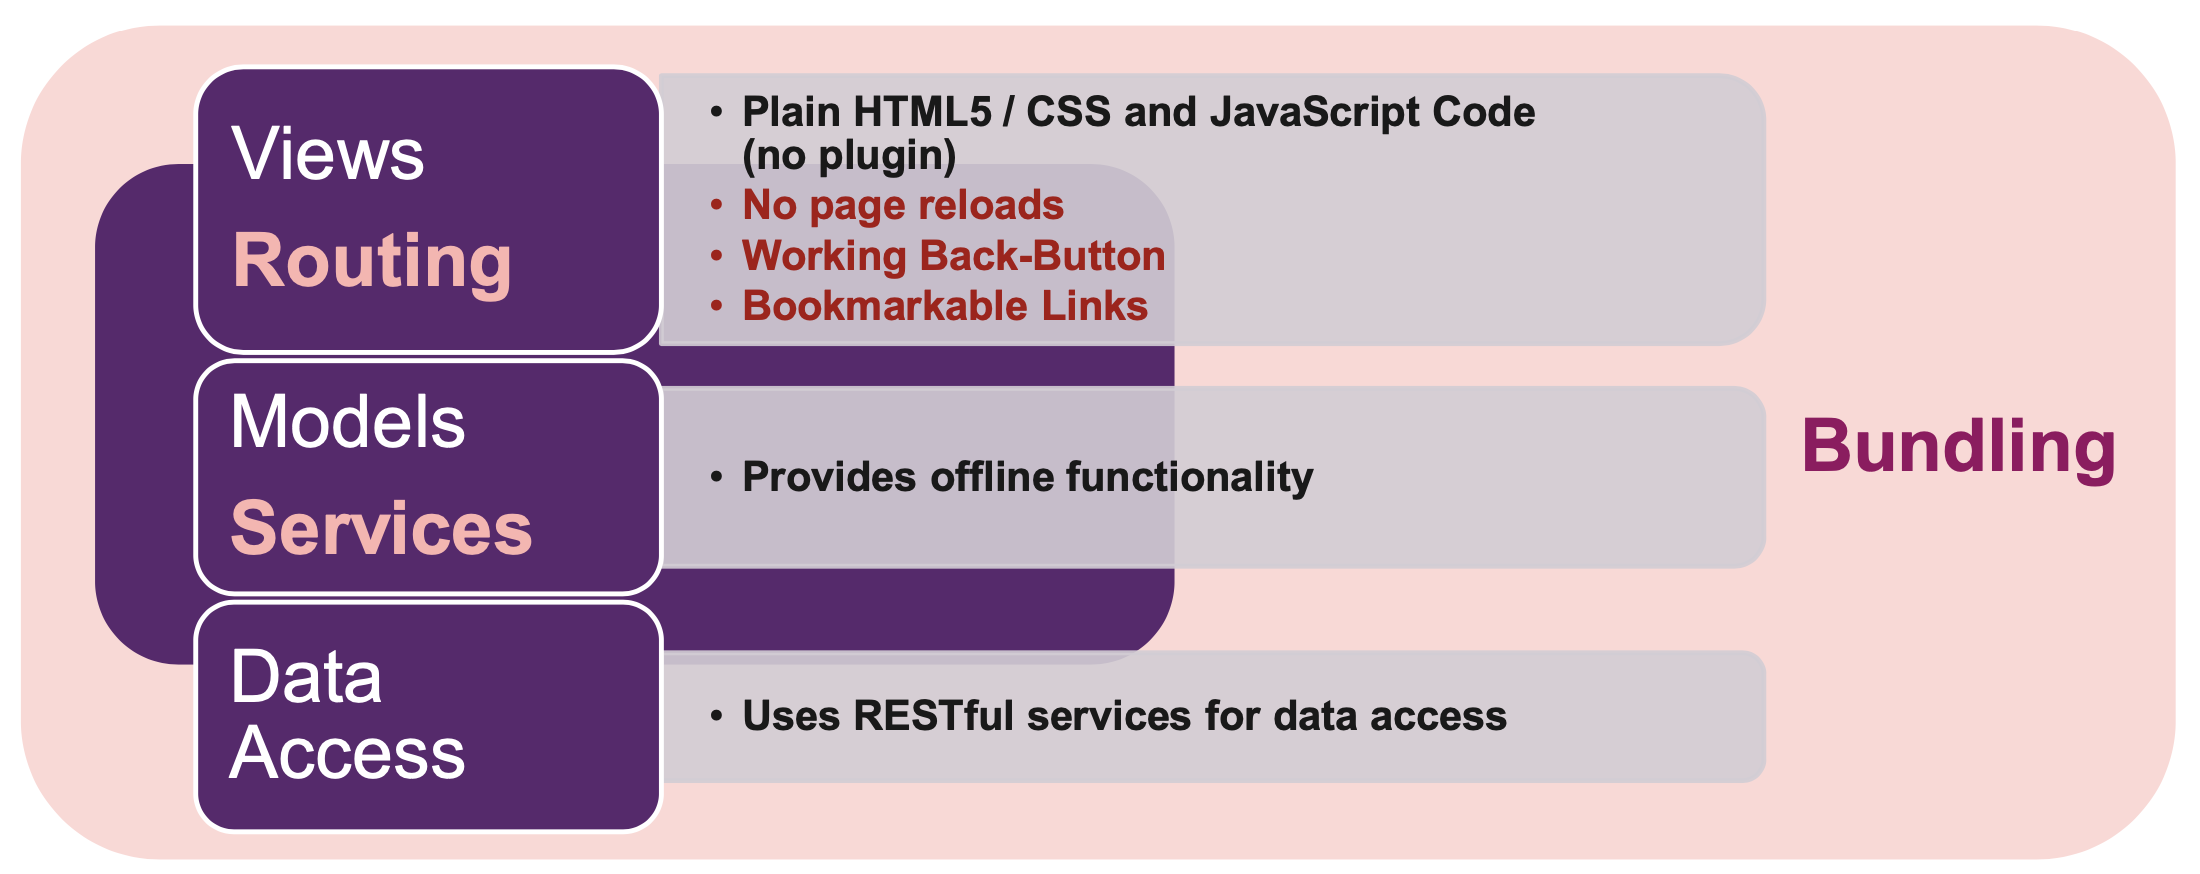
\includegraphics[width=\linewidth]{spa_logical_overview}

        \textbf{Bundeling}: Gesamter JavaScript-Code muss über tendenziell langsame Leitung zu Kunden, bundling und minifying reduziert Grösse, grosse SPAs brauchen vernünftiges Dependency Management, Module können auch On-Demand geladen werden, Bundler kommen und gehen (z.B. Webpack, Grunt, Rollup, esbuild)
        Webpack:

        \begin{itemize}
            \item Entry: Startpunkt wo Webpack mit Bundling beginnt und Dependencies findet.
            \item Output: Wo sollen die finalen Dateien hingeschrieben werden?
            \item Loaders: Transformiert Dateien in Module.
            \item Plugins: Können zusätzliche Funktionalitäten bieten (z.B. Asset Management)
            \item Mode: Aktivierung bestimmter Optimierungstechniken nach Bedarf.
        \end{itemize}

        \textbf{Routing}: Wird in SPAs komplett client-seitig gemacht, Browser "fakt" URL-Änderungen, Content muss für Zurück-Button persistiert werden.
        Früher gelöst mittels \#, heute mit \lstinline{window.history} / \lstinline{window.history.pushState}, verhindert das der Browser die URL wirklich lädt.
        Meistens gelöst über eine Routing-Tabelle, welche je nach verlangter Route eine andere Funktion aufruft.

        \textbf{Dependency Injection}: Reduziert Kopplung zwischen Konsument und Implementation, "Verträge" zwischen Klassen basieren auf Interfaces, erlaubt flexible Ersetzung einer konkreten Implementieren.


        \section{React}

        Eine Bibliothek, kein Framework!
        Umfasst nur das V aus MVC.
        \textbf{Prinzip von React}: Komplexe Probleme in kleinere Komponenten aufteilen.
        Verbessert Wiederverwendbarkeit, Erweiterbarkeit, Wartbarkeit, Testbarkeit, Aufgabenverteilung im Team.

        \textbf{JSX}: React-Komponenten sind Funktionen, welche HTML zurückgeben können (JSX).
        JSX kann an beliebigen Stellen verwendet werden, wenn Dateiendung stimmt.
        In eckigen Klammern stehen dann JavaScript-Expresssions.
        Einschränkung: React-Elemente müssen mit Grossbuchstaben starten, \lstinline{className} anstatt \lstinline{class} verwenden wegen gesperrter Keywords.
        Unterelement sind mittels \lstinline{props.children} zugänglich.
        \lstinline{props} als read-only behandeln!

        \begin{lstlisting}
        function Container(props) {
            return (
            <div className="container">
                {props.children}</div>
            )
        }

        function App() {
            return (
                <Container><HelloMessage name="OST"/></Container>
            )
        }
        \end{lstlisting}

        Styles werden als Objekt übergeben, muss Camel Case verwenden (\lstinline{min-height} wird zu \lstinline{minHeight}).
        Die JSX-Elemente werden zu \lstinline{React.createElement} umgewandelt, daher muss in jedem JSX-File React importiert werden, auch wenn es nicht aktiv verwendet wird.

        \begin{lstlisting}
        function Container(props) {
          return React.createElement("div",
            { className: "container" },
            props.children
          )
        }
        \end{lstlisting}

        React-Kompontenten konnten früher mittels Klasse definiert werden.
        Seit den Hooks aber nicht mehr nötig.

        \begin{lstlisting}
        class HelloMessage extends React.Component {
          render() {
            return <div>Hello {this.props.name}</div>
          }
        }
        \end{lstlisting}

        Anlegen einer neuen App: \lstinline{npx create-react-app hello-ost}.
        Konfiguration kommt dann aus einem NPM-Paket (Webpack, Babel, etc.).
        Kann mittels \lstinline{eject} entfernt werden.

        \textbf{Mount}: Komponenten müssen mittels Instruktion gemountet werden.
        Theoretisch mehrere Mounts pro Webseite möglich.

        \begin{lstlisting}
        import React from 'react';
        import ReactDOM from 'react-dom/client';
        import App from './App';

        const root = ReactDOM.createRoot(document.getElementById('root')); root.render(<App />);
        \end{lstlisting}

        \textbf{State}: Mittels \lstinline{useState} Hook.
        \lstinline{useState} müssen immer in derselben Reihenfolge erfolgen, somit if-Konditionen nicht möglich.
        State einer Komponente ist immer privat, kann aber als Props weitergegeben werden.
        Auch Event-Handler / Setter können als Props an Komponenten weiter gegeben werden.
        Zustand darf ausschliesslich mit Settern geändert werden.

        \begin{lstlisting}
        import { useState } from 'react';

        function Counter() {
          const [counter, setCounter] = useState(0);
          const increment = () => setCounter(counter + 1);
          return (
            <div>
              <p>{counter}</p>
              <button onClick={increment}>Increment Counter</button> </div>
          )
        }
        \end{lstlisting}

        \textbf{Reconciliation}: React-Komponenten werden als virtueller DOM gerendert, Wird der State geändert, erstellt React einen neuen virtuellen DOM, alter und neuer DOM werden verglichen, erst dann werden geänderte DOM-Knoten im Browser erstellt.

        \textbf{Formulare}: Event Handler bei den Inputs registrieren und Zustand ändern.

        \begin{lstlisting}
        <input value={username} type="text" onChange={e => setUsername(e.target.value)} />
        \end{lstlisting}

        Oder mittels \lstinline{onSubmit} auf dem Formular abfangen.

        \begin{lstlisting}
        function handleSubmit(event) {
            event.preventDefault();
            alert("Username: " + username + ", Password: " + password)
        }
        \end{lstlisting}

        \textbf{Styling}: Meistens mittels Widget-Library, z.B. Reactstrap, Material UI oder Semantic.

        \textbf{Lifecycles}: Klassenkomponenten haben eine Reihe an Lifecycle-Methoden wie \lstinline{componentDidMount} , \lstinline{shouldComponentUpdate(nextProps, nextState)} oder \lstinline{componentWillUnmount}.
        Mit Hooks vereinfacht mit \lstinline{useEffect}.
        \lstinline{useEffect} kann mit Promises verwendet werden.

        \begin{lstlisting}
        useEffect(() => {
          const timerID = setInterval(() => setDate(new Date()), 1000) // ausgefuehrt beim Mount
          return () => {
            clearInterval(timerID) // ausgefuehrt beim Unmount
          }
        }, []) // Arrays von Dependencies, kann genutzt werden, um Effekt auszuloesen, wenn sich Abhaengigkeit aendert
        \end{lstlisting}

        \textbf{Routing}: Mittels React Router (Kollektion von Navigationskomponenten für React, für Web und Native).
        Alle Router müssen Teil von \lstinline{<BrowserRouter>} sein.
        \lstinline[mathescape]!<Route path="/about" element ={<About/>} />!: Component About wird nur gerendert, wenn der path matcht.
        App-interne Links verwenden nicht <a> sondern <Link>. \lstinline[mathescape]!<Link to="/about">About</Link>!

        \textbf{Type-Checking}: Flow erweitert JavaScript um Typannotationen.
        Lieber Typescript für mehr Typsicherheit in React-Komponenten.
        Flow sind nur Annotations, können daher einfach ignoriert werden, Typescript ist eine ganze Programmiersprache.

        \textbf{React Context}: Daten immer als Props mitgeben ist mühsam, Zustand verteilt sich über gesamte Applikation, Calls sind auch verteilt.
        React Context ermöglicht es, Props für alle Unterkomponenten zur Verfügung zu stellen.

        \begin{lstlisting}
        const ThemeContext = React.createContext(themes.light);

        function App() {
          return (
            <ThemeContext.Provider
              value={themes.dark}>
              <Toolbar />
            </ThemeContext.Provider>
          );
        }

        function ThemedButton() {
          const theme = useContext(ThemeContext);
          return (
            <button style={{
              background: theme.background,
              color: theme.foreground
            }}>
              {" "}I am styled by theme context!{" "}
            </button>
          );
        }
        \end{lstlisting}

        \textbf{Redux}: Darstellung des States als Baum, Baum ist nicht veränderbar, Veränderungen am Baum führen zu einem neuen Baum, Verwaltung über Stores.

        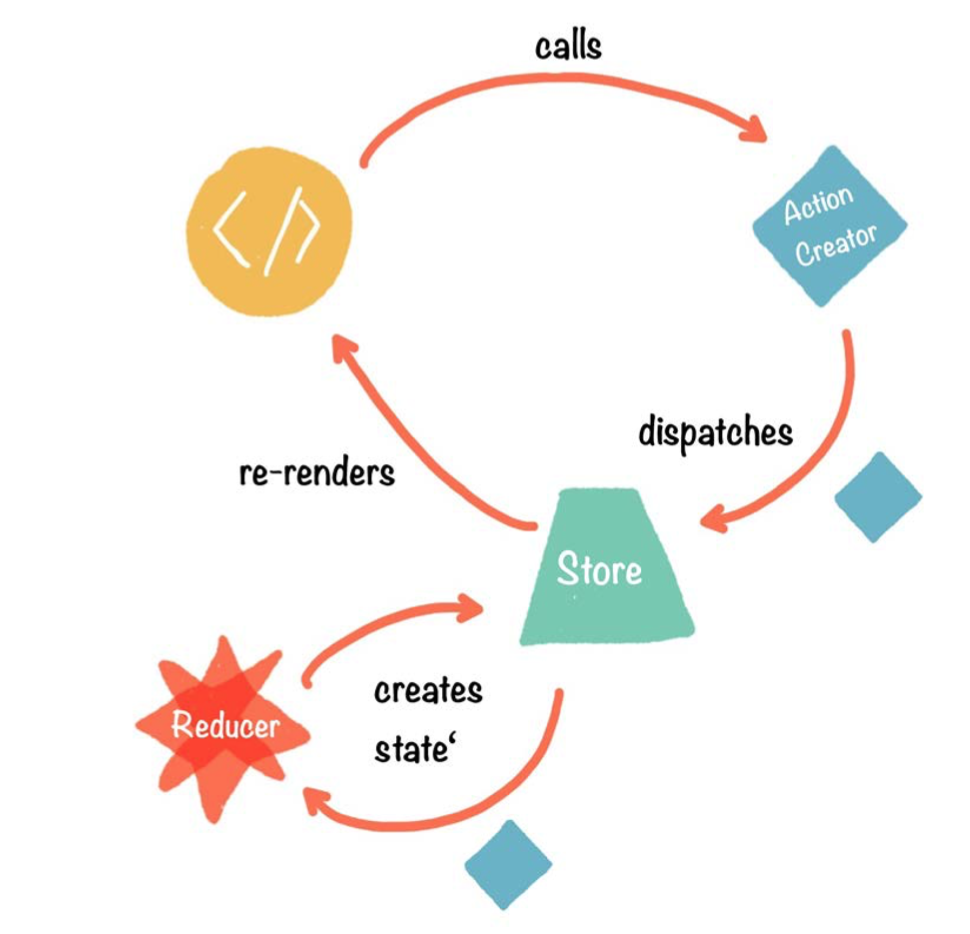
\includegraphics[width=\linewidth]{redux_data_flow}

        Eine Veränderung braucht eine Action (sehr simple Objekte wie \lstinline!{ type: 'TRANSFER', amount: 100 }!).
        Der Store braucht einen Reducer, um mit der Action den neuen Baum zu machen.
        Reducer sind pure Funktionen ohne Seiteneffekte.

        Soll / Muss in jeder React-Applikation Redux eingesetzt werden?
        Nein, wenn kaum Zustand existiert, der von mehreren Komponenten verwendet wird, lohnt sich der Redux-Overhead nicht.

        \begin{lstlisting}
        function balance(state = 0, action) {
          switch (action.type) {
            case 'TRANSFER':
              return (
                state + action.amount
              )
            default:
              return state
          }
        }
        \end{lstlisting}

        Mehrere Reducer bilden einen Root Reducer.
        Initialer State für die App ist ein leeres Objekt.

        \begin{lstlisting}
        function rootReducer(state = {}, action) {
          return {
            balance: balance(state.balance, action),
            transactions: transactions(state.transactions, action)
          }
        }

        // gleichwertig
        const rootReducer = combineReducers({
           balance,
           transactions
        })

        const store = createStore(rootReducer);
        \end{lstlisting}

        Über Änderungen am State kann man sich mittels Listener benachrichtigen lassen: \lstinline{store.subscribe(() => console.log(store.getState()));}

        \textbf{React und Redux}: Redux Toolkit verwenden.
        \lstinline{createSlice} erstellt neue Stateobjekte, Reduce-Funktionen und Aktionen.
        Action-Type im unteren Beispiel ist \lstinline{balance/transfer}.
        Mittels immer.js scheinbare, direkte Änderungen am State möglich.

        \begin{lstlisting}
        const balanceSlice = createSlice({
          name: "balance",
          initialState: { value: 0 },
          reducers: {
            transfer: (state, action) => {
              state.value += action.payload.amount;
            },
          },
        });
        export const { transfer } = balanceSlice.actions;
        \end{lstlisting}

        \lstinline{configureStore} initialisiert den Redux Store mit den angegeben Reducern.
        Enthält \lstinline{redux-thunk}.
        Redux Thunk erlaubt es uns, anstelle eines Objektes eine Funktion zu dispatchen.

        \begin{lstlisting}
        const store = configureStore({
          reducer: { balance: balanceReducer }
        });
        \end{lstlisting}

        Verfügbarkeit in React-Applikation mittels Provider.

        \begin{lstlisting}
        render(
          <Provider store={store}>
            <App />
          </Provider>,
          document.getElementById('root')
        )
        \end{lstlisting}

        \lstinline{useDispatch} wird für den Dispatch der Aktionen an den Store benutzt.
        \lstinline{useSelector} wird für die Abfrage des States benutzt.

        \begin{lstlisting}
        const dispatch = useDispatch()
        dispatch(transfer({ amount: 10 }))
        const balance = useSelector(state => state.balance.value);
        \end{lstlisting}

        Asynchrone Actions:

        \begin{lstlisting}
        // First, create the thunk
        export const transferAsync = createAsyncThunk(
          "balance/transferApiRequest",
          async (amount) => {
            const response = await api.transfer(amount);
            return response.data;
          }
        );

        const balanceSlice = createSlice({
          initialState: { value: 0, status: "idle" },
          extraReducers: (builder) => {
            builder
              .addCase(transferAsync.pending, (state) => {
                state.status = "loading";
              })
              .addCase(transferAsync.fulfilled, (state, action) => {
                state.status = "idle";
                state.value += action.payload.amount;
              });
          },
        });
        \end{lstlisting}

        \textbf{JHipster}: Fullstack App-Generator mit Angular, React-Redux oder Vue, Spring Boot, Maven/Gradle, NPM, Postgres, MongoDB, Elasticsearch, Cassandra, Kafka etc.
        Bieten eigene DSL für Entities und Relationen.

        \textbf{Testing}: Jest offizielle Lösung von Facebook, kommt mit \lstinline{create-react-app} mit.
        Die React Testing Library baut auf der DOM Testing Library auf und fügt APIs für die Arbeit mit React-Komponenten hinzu.
        JHipster generiert End-to-End-Tests mit Cypress.

        \begin{lstlisting}
        import { render, screen } from '@testing-library/react'
        import userEvent from '@testing-library/user-event'

        test('loads and displays greeting', async () => {
          // ARRANGE
          render(<Fetch url="/greeting" />)

          // ACT
          await userEvent.click(screen.getByText('Load Greeting'))
          await screen.findByRole('heading')

          // ASSERT
          expect(screen.getByRole('heading')).toHaveTextContent('hello there')
          expect(screen.getByRole('button')).toBeDisabled()
        })
        \end{lstlisting}


        \section{Angular}

        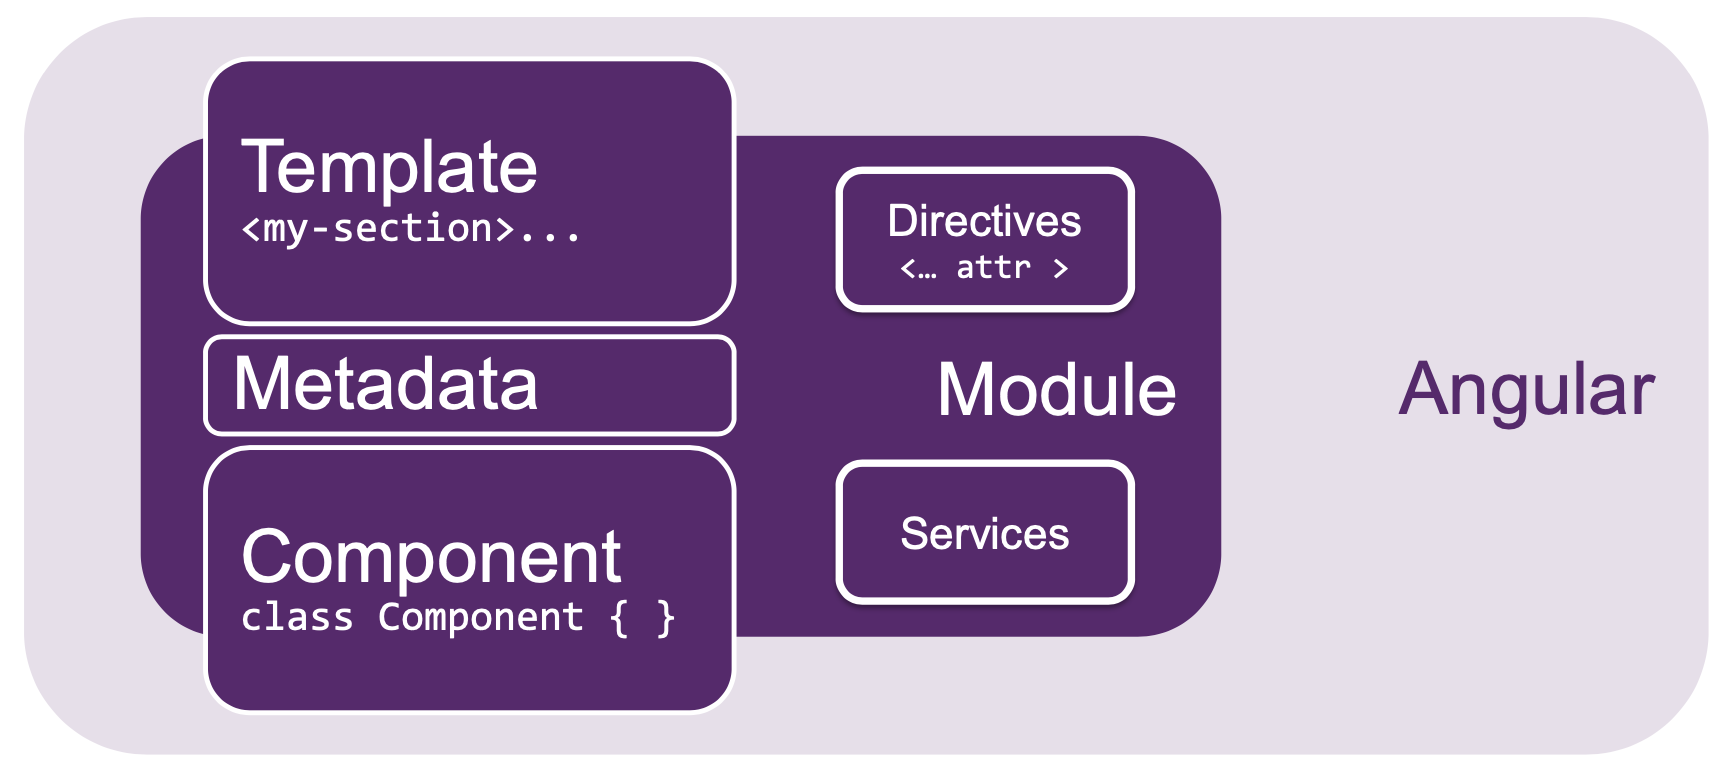
\includegraphics[width=\linewidth]{base_angular}

        TypeScript-basiert, mit Dependency Injection, 2-Way-Bindings, klar strukturiert.
        Sollte verwendet werden für lang lebende und komplexe Applikationen.
        Historie: Modernes Angular seit v2, v1 wird AngularJS genannt, keine Gemeinsamkeiten.
        v3 ausgelassen, um Paketnamen zu harmonisieren.
        \lstinline{npx ng new my-app} legt neue Applikation an (Paket lokal installieren mit \lstinline{npm install @angular/cli})

        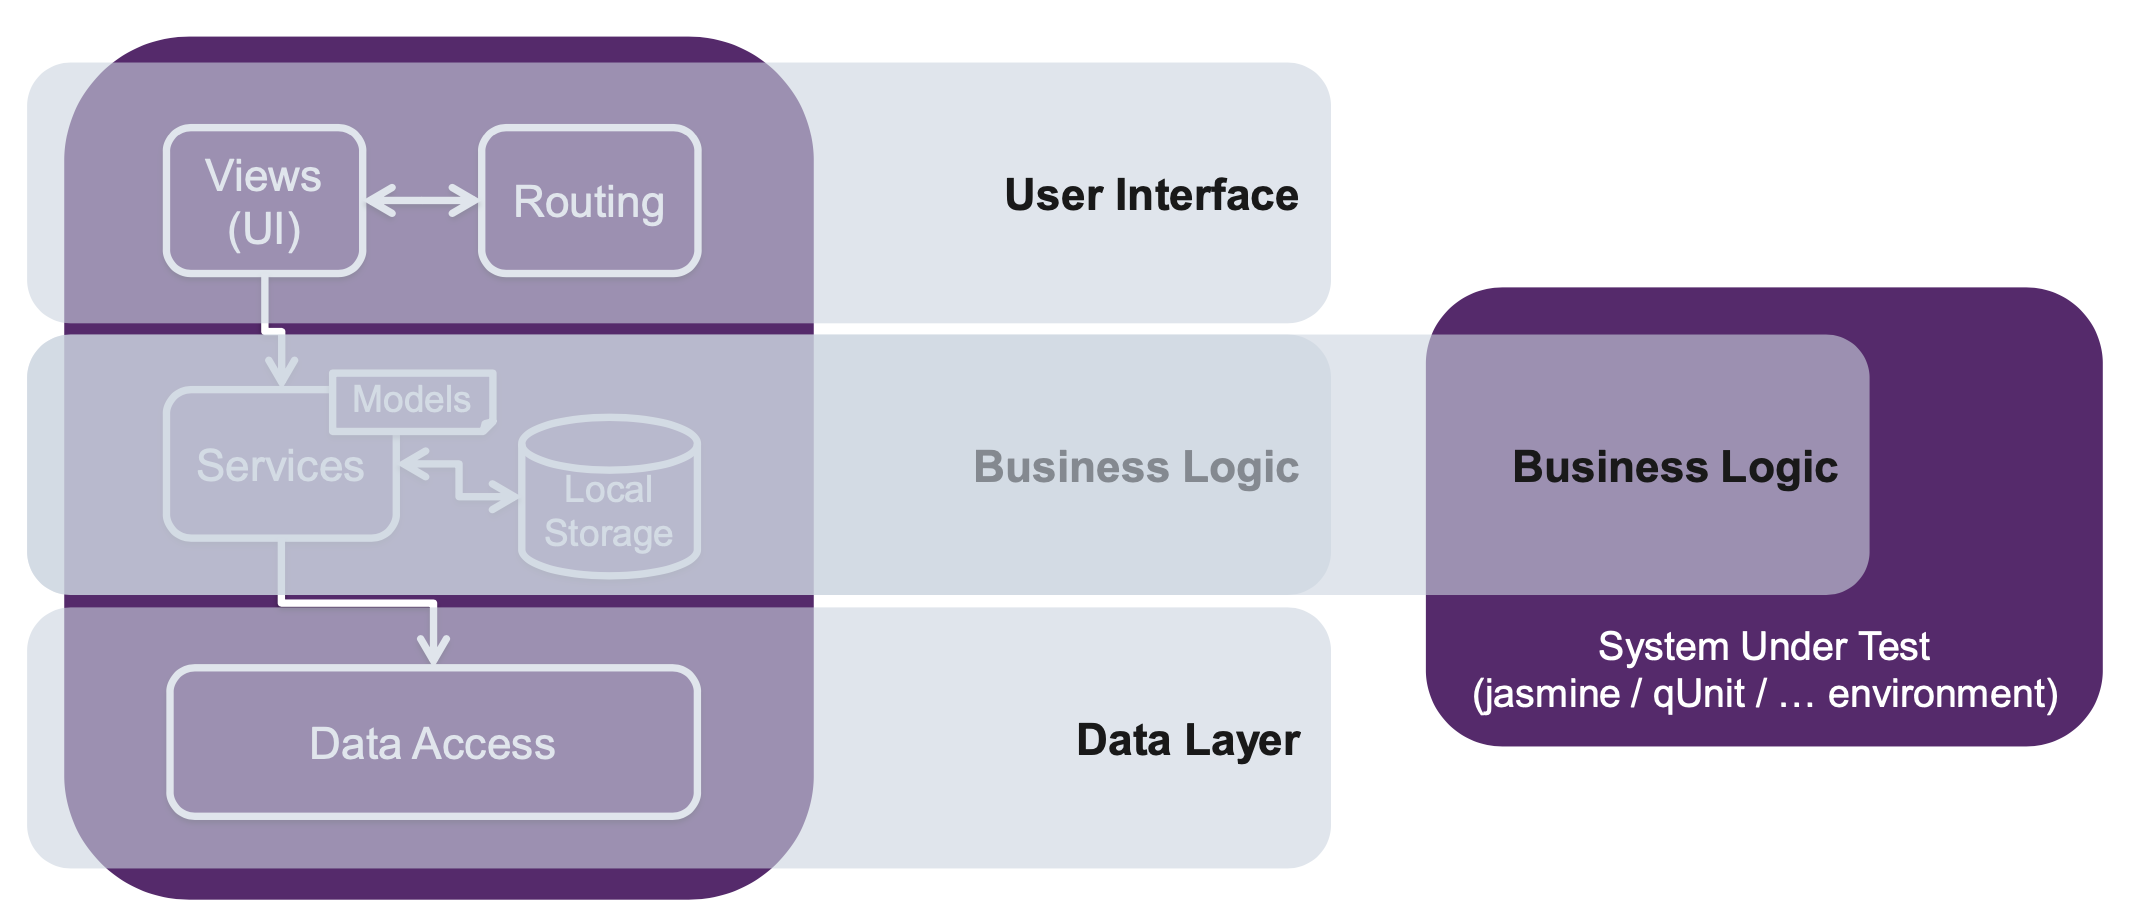
\includegraphics[width=\linewidth]{angular_logical_layers}

        \textbf{Dependency Injection}: Registration beim Container, Request, Resolve durch Container, Fullfill (TypeScript module/s).
        \textbf{ngModules}: Ein zusammenhängender Codeblock, der eng miteinander verbundenen Fähigkeiten gewidmet ist (TypeScript class).
        Jede App hat mindestens ein Modul, das Root-Modul.
        Exportieren Features wie Services oder Direktive für andere Module.
        ngModule-Deklaration selbst wird in ein TypeScript-Modul eingefügt (meistens über \lstinline{index.ts}).

        \begin{lstlisting}
        @NgModule({
            exports: [] // The subset of declarations that should be visible and usable in the component templates of other modules.
            imports: [CommonModule], // Specifies the modules which exports/providers should be imported into this module.
            declarations: [], // The view classes that belong to this module (components, directives and pipes).
            providers: [], // Creators of services that this module contributes to the global collection of services (Dependency Injection Container); they become accessible in all parts of the app.
            bootstrap: [] // The main application view, called the root component. Only the root module should set this property.
        })

        export class CoreModule { }
        \end{lstlisting}

        \textbf{Module-Importe}: Standardmässig wird alles aus dem Modul importiert und Dependency-injected.
        \lstinline{forChild(config?)}: Statische Methode auf dem Modul, erlaubt Services für den aktuellen Modul-Level zu konfigurieren.
        \lstinline{forRoot(config?)}: Statische Methode auf dem Modul, injected und konfiguriert Services global.
        Nur im Root-Modul machen!
        \lstinline{providedIn: 'root'} bevorzugen, wenn Services keine Konfiguration benötigen.

        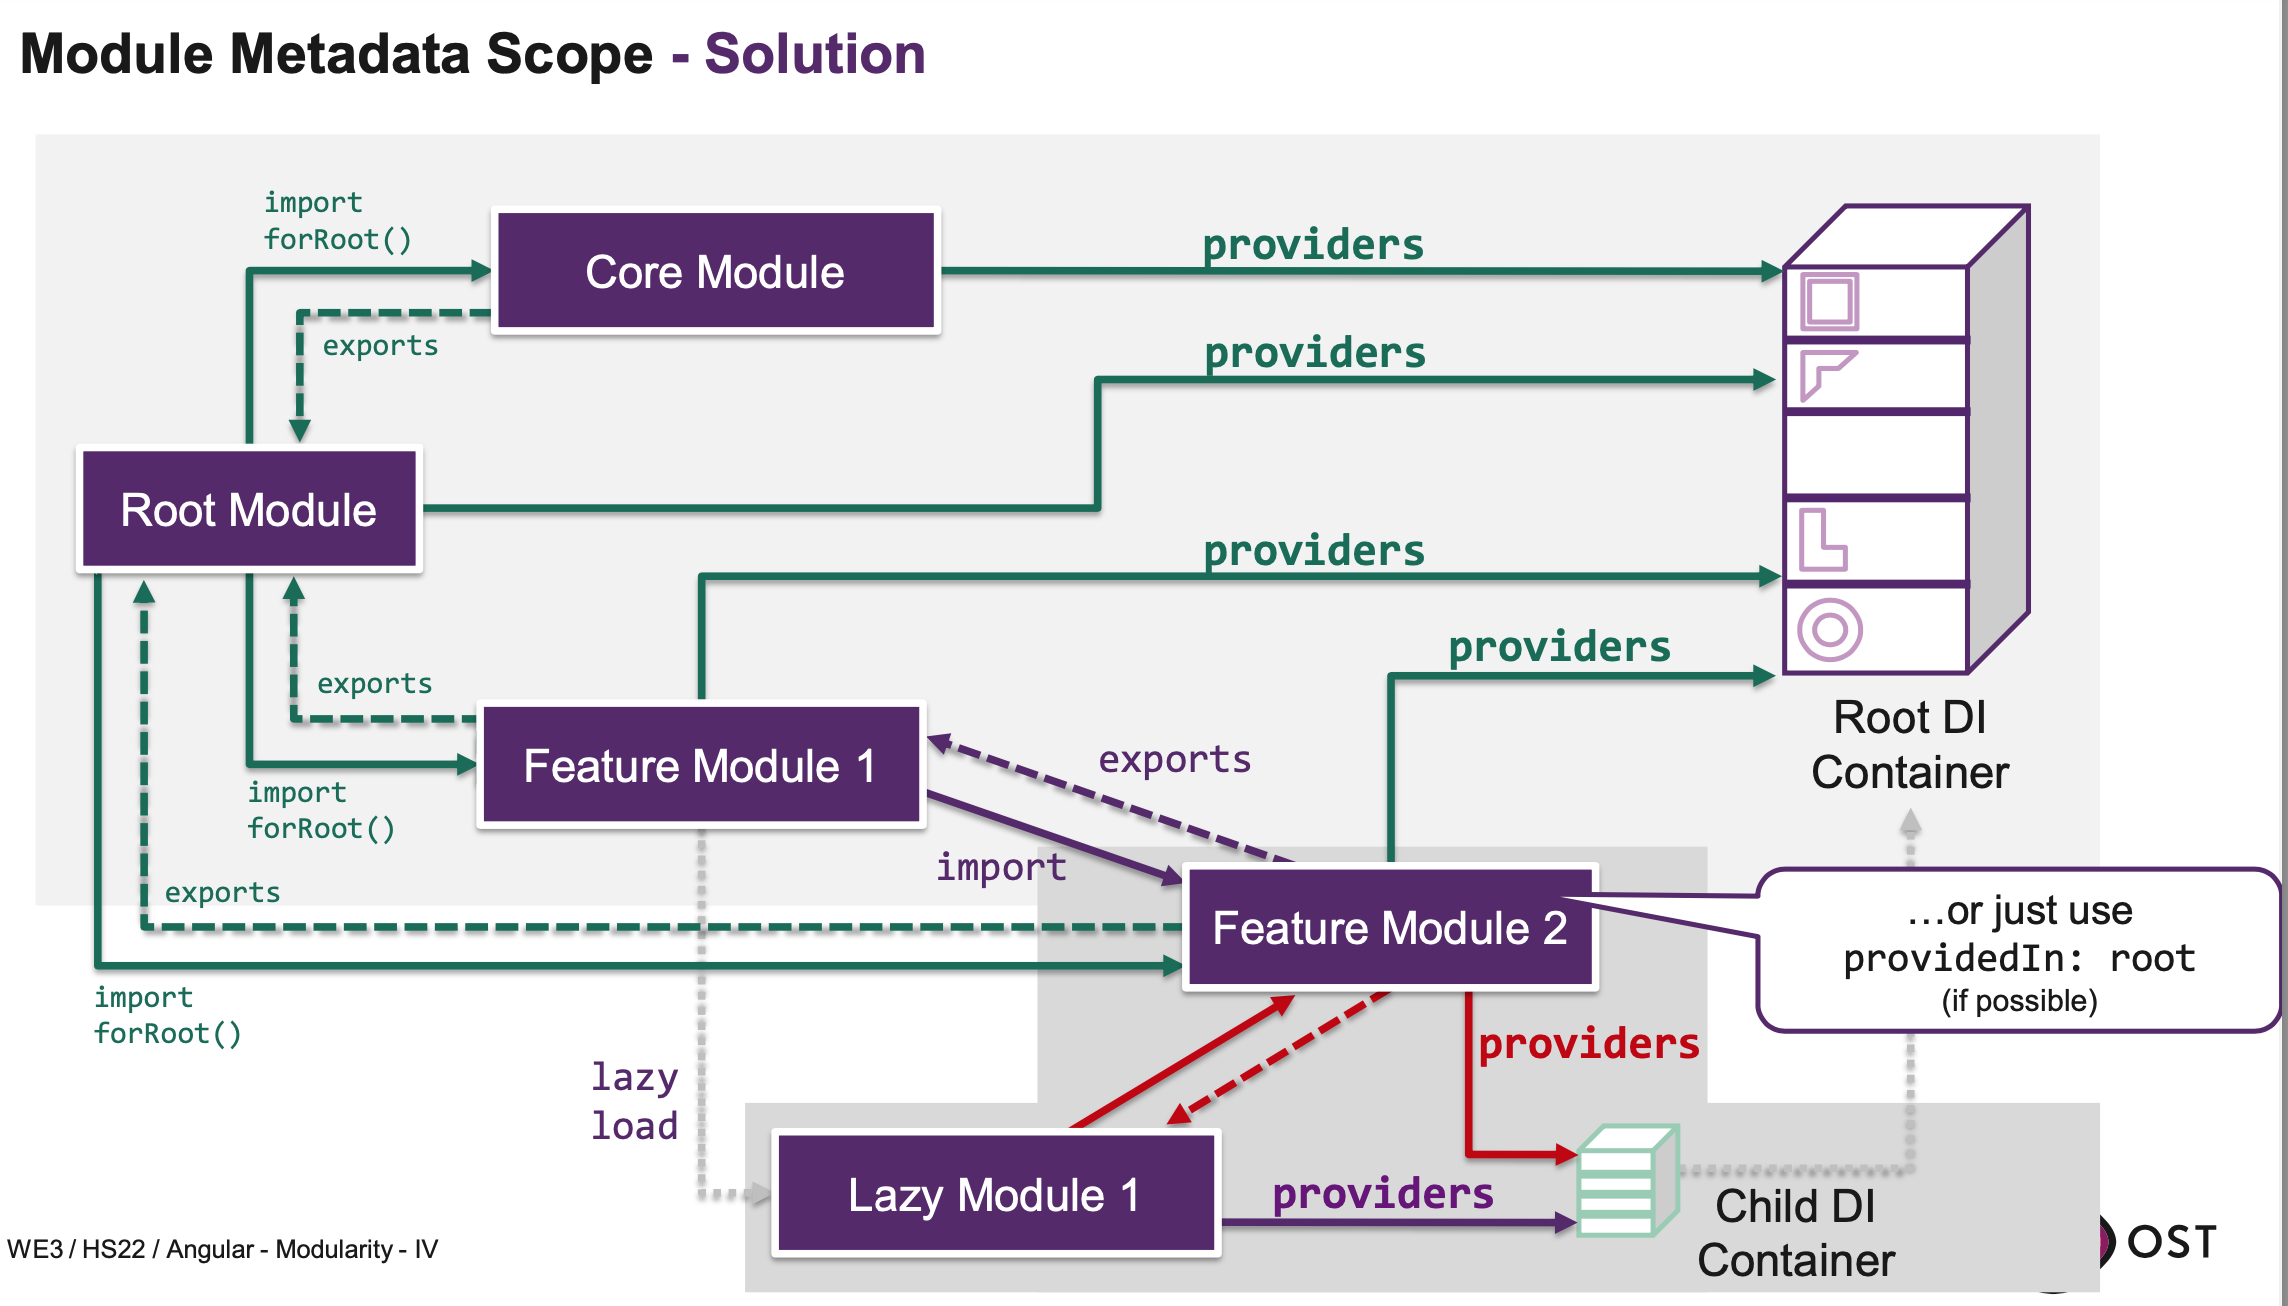
\includegraphics[width=\linewidth]{angular_module_big_picture}

        \textbf{Modultypen}: Root / App Modul: Einstiegspunkt in die Applikation.
        Exportiert nichts.
        Konventionell AppModule genannt und existiert in einer Datei namens app.module.ts.
        Importiert BrowserModule, die jede Browser-Anwendung importieren muss

        \textbf{Feature-Modul}: Teile der Applikation.
        Es ist die beste Praxis, Feature-Module in Domain-, Routing-, Service-, Widget- und Lazy-Module aufzuteilen (siehe unten).
        Ermöglicht die Zuweisung von Entwicklungsaufgaben an verschiedene Teams.

        \textbf{Shared-Modul}: "Toolkit" der Applikation, alles was irgendwie in kein Modul passt.
        Keine app-weiten Singleton-Anbieter (Dienste) in einem gemeinsamen Modul angeben.

        \textbf{Core-Modul}: Initialisiert globale Services.
        Ein "lazy-loaded"-Modul, das dieses gemeinsame Modul importiert, erstellt seine eigene Kopie des Dienstes.
        Wird nur vom Root-Modul importiert, der Import in ein anderes Modul, insbesondere in ein "Lazy-Load"-Modul, widerspricht der Absicht und kann zu einem Laufzeitfehler führen.

        \textbf{Lazy Modules}: Ähnlich wie Feature-Modules, werden aber lazy loadet wenn angefragt mittels Dependency Injection.

        \textbf{Feature-Modul-Untertypen}: Domain-Modul: Bereitstellung einer auf einen bestimmten Anwendungsbereich zugeschnittenen Benutzeroberfläche.
        Routing-Modul: Gibt die Routing-spezifischen Konfigurationseinstellungen des Feature- (oder Root-) Moduls an.
        Service-Modul: Bietet Versorgungsdienste wie Datenzugriff und Nachrichtenübermittlung.
        Widget Modul: Macht Komponenten, Direktiven und Pipes für externe Module verfügbar.

        \textbf{Directives}: Enthält Anweisungen zur Transformation des DOM (TypeScript class).
        Besitzen kein Template.
        Brauchen \lstinline{@Directive()}-Decorator.
        Structural directives: Verändern DOM.
        Diese werden im Hintergrund zu \lstinline{<ng-template>} umgewandelt.
        \lstinline{<ng-template>} kann auch verwendet werden, wenn kein HTML-Element benötigt wird.
        \lstinline{<ng-template>} können nicht mit weiteren Structural directives verwendet werden.
        Attribute directives: Ändern des Aussehens oder Verhaltens eines vorhandenen Elements.

        \begin{lstlisting}
        <div *ngIf="hasTitle"><!-- shown if title available --></div>
        <div [ngStyle]="{ 'font-size': isSpecial ? 'x-large' : 'smaller' }">
                 <!-- render element -->
        </div>
        \end{lstlisting}

        \textbf{Template Reference Variables}: Verfügbar im gesamten Template.

        \begin{lstlisting}
        <input placeholder="phone number" #phone>
        <button (click)="callPhone(phone.value)">Call</button>
        \end{lstlisting}

        \textbf{Components}: Eine Komponente ist eine Richtlinie mit einer Vorlage; sie steuert einen Abschnitt der Ansicht (HTML File / (S)CSS / \ldots).
        Basiert auf MVC oder MVVM.
        Eine Komponente sollte so klein und zusammenhängend wie möglich implementiert werden, um die Testbarkeit / Wartbarkeit / Wiederverwendbarkeit zu unterstützen.
        Komponenten kontrollieren die View (genau eine View pro Komponente).
        Mittels Selektor kann Komponent in anderen Views verwendet werden (entweder tag-name oder CSS-Selektor ( id-selector \#topHeader)), braucht Registierung im ngModule bei \lstinline{declarations} und \lstinline{exports}.
        Lifecycle wird verwaltet von Angular (Hydration, Update, Dehydration), können mittels Methoden wie \lstinline{ngOnInit} und \lstinline{ngOnDestroy} erweitert werden.
        Komponent braucht Deklaration wie \lstinline{implements OnInit, OnDestroy}, damit Methoden verwendet werden können.
        View-Code muss gültiges HTML5 sein.

        \begin{lstlisting}
        <p>Your team is <strong>{{counter.team}}</strong></p>
        <p>Your current count is
            <strong>{{counter.count}}</strong>
        </p>
        <form>
            <button (click)="up($event)">Count Up</button>
        </form>

        @Component(...)
        export class CounterComponent implements OnInit {
            counter: CounterModel = new CounterModel(); up(event: UIEvent): void {
                this.counter.count++;
                event.preventDefault();
            }
        }
        \end{lstlisting}

        \textbf{Bindings}: Two Way Binding / Banana in a box [( ... )].
        One Way (from View to Model / Event Binding) ( ... ).
        One Way (from Model to View / Property Binding) [ ... ] or {{ ... }}.

        \begin{lstlisting}
        public counter: any = {
            get team() { return null }, set team(val) { }, eventHandler: () => { }
        }

        <input type="text" [(ngModel)]="counter.team">
        <button (click)="counter.eventHandler($event)">
        <p>... {{counter.team}} ..</p>
        \end{lstlisting}

        Die Bindung an Ziele muss als Inputs oder Outputs deklariert werden.

        \begin{lstlisting}
        @Component({...})
        export class NavigationComponent {
            @Output() click = new EventEmitter<any>();
            @Input() title: string;
        }

        <wed-navigation(click)="..."[title]="..."></wed-...>
        \end{lstlisting}

        \textbf{Metadata}: Metadaten beschreiben eine Klasse und sagen Angular, wie sie zu verarbeiten ist (TypeScript decorator).

        \textbf{Services}: Bietet Logik für jeden Wert, jede Funktion oder jedes Merkmal, das Ihre Anwendung benötigt (TypeScript class).
        Werden mittels Dependency Injection erstellt, wenn Komponenten Service-Abhängigkeit deklarieren.
        \textbf{Service-Kommunikation mit UI}: Theoretisch alles mittels RxJS möglich, in WED3 aber mit \lstinline{EventEmitter} behandelt (siehe oben).
        RxJS implementiert das Observer-Pattern für JavaScript.
        \textbf{Hot Observables}: Sequenz von Events wie Mausklicks, verfügbar für alle Subscriber.
        \textbf{Cold Observables}: Starten erst bei ersten Subscriber, schliessen sobald Task beendet.
        \textbf{Data Resources}: Abstrahieren HTTP-Kommunikation, um Daten abzuholen.
        Jeweils \lstinline{HttpClient} verwenden, verwendet Cold Observerables.

        \begin{lstlisting}
        export class SampleModel { }

        @Injectable({ providedIn: 'root')
        export class SampleService {
            private samples: SampleModel[] = []; // simple cache
            public sampleChanged: EventEmitter<SampleModel[]> = new EventEmitter<SampleModel[]>();
            constructor(
                private dataResource: SampleDataResourceService) {
            }
            load(): void {
                this.dataResource.get().subscribe(
                    (samples: SampleModel[]) => { // update cache, emit change event, ...
                        this.samples = samples;
                        this.sampleChanged.emit(this.samples);
                    });
            }
        }

        @Component({ ... })
        export class SampleComponent implements OnInit, OnDestroy {
            private samples: SampleModel[];
            private samplesSubscription: Subscription;
            constructor(private sampleService: SampleService) { }

            ngOnInit() {
                this.samplesSubscription = this.sampleService.samplesChanged.subscribe(
                    (data: SampleModel[]) => { this.samples = data; });
            }

            ngOnDestroy() {
                this.samplesSubscription.unsubscribe();
            }
        }
        \end{lstlisting}

        HTTP-Requests können abgefangen und modifiziert werden.

        \begin{lstlisting}
            @NgModule({ ...})
            export class SampleModule {
                static forRoot(config?: {}): ModuleWithProviders {
                    return {
                        ngModule: SampleModule,
                        providers: [
                            {
                                provide: HTTP_INTERCEPTOR,
                                useClass: AuthInterceptor,
                                multi: true
                            }
                        ]
                    }
                }
            }

            @Injectable()
            export class AuthInterceptor implements HttpInterceptor {
                constructor(private store: SecurityTokenStore) { }

                public intercept(req: HttpRequest<any>, next: HttpHandler) {
                    const authReq = req.clone({
                        setHeaders: {
                            Authorization: `Bearer ${this.store.token}`
                        },
                        withCredentials: true
                    });

                    return next.handle(authReq);
                }
            }
        \end{lstlisting}

        \textbf{Template-driven forms}: Angular Template-Syntax mit den formularspezifischen Direktiven und Techniken.
        Erzeugt weniger Code, platziert aber die Validierungslogik in HTML.
        \textbf{Reactive (or model-driven) forms}: Import von \lstinline{ReactiveFormsModule} nötig, Form und Validations werden im Controller gebaut, mehrere asynchrone Validierungen möglich.
        Nicht Teil der Lektüre!

        \begin{lstlisting}
        <form (ngSubmit)="doLogin(sampleForm)" #sampleForm="ngForm">
            <input type="text" class="form-control" id="name" required [(ngModel)]="model.name" name="name" #nameField="ngModel">
            <div [hidden]="nameField.valid || nameField.pristine" class="alert alert-danger">
                Name is required
            </div>

            <button type="submit" class="btn btn-success" [disabled]="!sampleForm.form.valid">Submit</button>
        </form>

        @Component({ ... })
        export class SampleComponent {
            public doLogin(f?: NgForm): boolean {
                if (f?.form.valid) { // store data
                    Component
                    return false; // avoid postback }
                }
            }
        }
        \end{lstlisting}

        \textbf{Component Transclusion / Content Projection}: Selbiges wie Reacts \lstinline{props.children}.

        \begin{lstlisting}
        <wed-navigation>
            <h1 wed-title>WED3 Lecture</h1>
            <menu><!-- ... --></menu>
        </wed-navigation>

        <header>
            <ng-content select='[wed-title]'> </ng-content>
        </header>
        <nav>
            <ng-content select='menu'>
            </ng-content>
        </nav>

        <wed-navigation>
            <header>
                <h1 wed-title>WED3 Lecture</h1>
            </header>
            <nav>
                <menu><!-- ... --></menu>
            </nav>
        </wed-navigation>
        \end{lstlisting}



        \begin{lstlisting}
        var subscription = this.http.get('api/samples').subscribe(
            function (x) { /* onNext -> data received (in x) */ },
            function (e) { /* onError -> the error (e) has been thrown */ },
            function () { /* onCompleted -> the stream is closing down */ }
        );
        \end{lstlisting}

        \textbf{Routing}: Routing Table mappt Routen zu Kompontenten.
        Oberste Routen registrieren mit \lstinline{forRoot()}, Subroutes mit \lstinline{forChild()}.
        \lstinline{forRoot()} kennt auch Router-Service, welcher Singleton ist in Applikation.
        Benötigt \lstinline{<base href="/">} im Header für relative URL oder \lstinline{APP_BASE_HREF} Variable.
        \lstinline{<router-outlet>} definiert, wo Routen angezeigt werden.
        \lstinline{'hero/:id'} ID ist hier eine Variable.
        \lstinline{redirectTo} erlaubt Weiterleitung.
        \lstinline{'**'} ist die Wild-Card-Route für 404.
        Routen werden aufgelöst nach "first come first served".
        Verschachtelung möglich mittels \lstinline{children}, Parent benötigt dann weiteres Router Outlet.

        \begin{lstlisting}
         const appRoutes: Routes = [
            {
                path: '', component: WelcomeComponent,
                children: [
                    { path: ':id', component: SamplesDetailComponent },
                ]
            },
            {
                path: 'config',
                loadChildren: () => import('./cfg/cfg.module').then(m => m.CfgModule), canLoad: [AuthGuard]
            }
        ];

         @NgModule({
            imports: [ RouterModule.forRoot(appRoutes) ],
            exports: [ RouterModule ]
         })
         export class AppRoutingModule {}
         \end{lstlisting}

        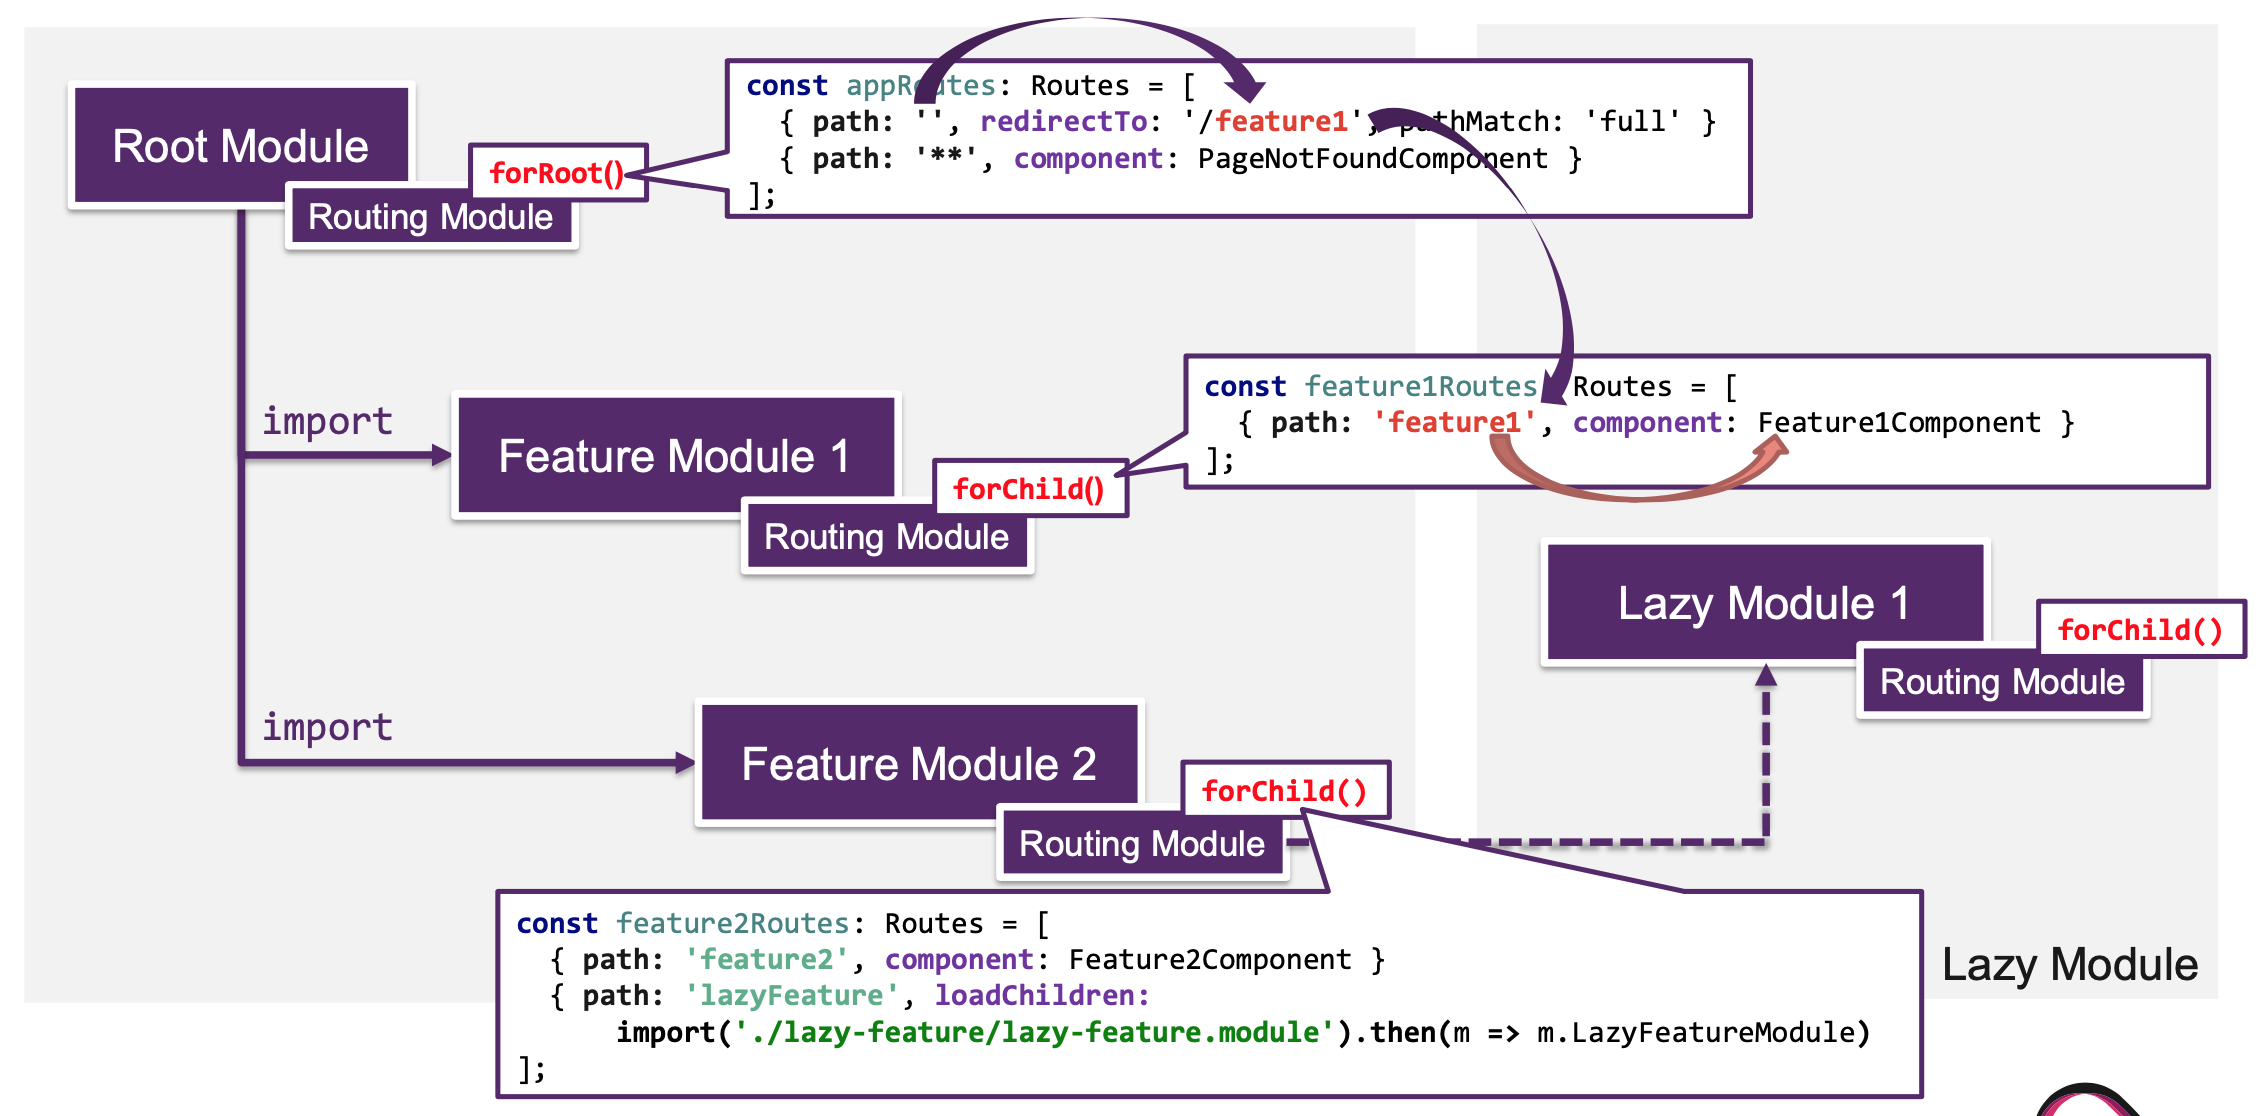
\includegraphics[width=\linewidth]{angular_routing}

        \section{.NET}
        Weshalb ASP.NET Core: Enterprise Framework, Kompilierbare Sprache (C\#), OS unabhängig.
        \textbf{Attribute}: intensiv eingesetzt (Um Konventionen zu übersteuern bzw zu unterstützen, Schnittstelle für Zusatzinformationen für Framework, Kann via "Reflection" ausgelesen werden).
        \begin{lstlisting}
          [Required]
          [StringLength(100, MinimumLength = 10)]
          public string Name {get; set; }

          [HttpPost]
          public ActionResult About()
        \end{lstlisting}
        % Asseembly.GetEntryassembly().GetTypes() -> Findet alle Typen mit einem bestimmten Attribut
        % Activator.CreateInstance(typesWithAttribute.First()) -> Erzeugt eine Instanz von diesem Type

        \textbf{Extension Methods}: C\# erlaubt es existierenden Klassen Methoden "hinzuzufügen"
        \begin{lstlisting}
          string s = "Hello Extension Methods";
          int i = s.WordCount();

          public static class MyExtensions
          {
            public static int WordCount(this string str) {
              return str.Split(new char[] {' ', '.', '?'}).Length;
            }
          }
        \end{lstlisting}

        \textbf{Async Await}
        \begin{lstlisting}
          static async Task Main(string[] args)
          {
            Console.WriteLine("--");
            await RunAsync();
            Console.WriteLine("--");
            Console.ReadLine();
          }

          public static Task<string> Send()
          {
            return Task.Run(() => {
              Console.WriteLine("Send!");
              return "nachricht gesendet";
            });
          }

          public static async Task<bool> RunAsync()
          {
            Console.WriteLine("Start Send");
            Console.WriteLine(await Send());
            Console.WriteLine("End Send");
            return true;
          }

          % outputs
          % -- start send send! nachricht gesendet end send -- 
        \end{lstlisting}
        \textbf{Convention over configuration (or coding by convention)}: seeks to decreasse the numbere of decision that developers need to make, gaining simplicity, and not necessarily losing flexibility.
        Nachteile: Magie, Ev. Schwer anzupassen (falls Anforderungen nciht inss Schema passen)
        \textbf{Multi-Threading}: Besitzt Thread Pool wo grösse konfigurierbar. Wählt für jeden Request einen Thread aus Pool für bearbeitung.
        Thread solange blockiert bis Request abgeschlossen (oder vorzeitig zurückgegeben -> async/await)
        Keine geteilten Daten in Controller / Services halten (z.B. Static Variablen, ASP.NET instanziert für jeden Request neuen Controller)
        \textbf{MVVM} View: Markup Language, was Benutzer sieht, Kommunikation zu ViewModel via Bindings. View Model: Daten für View aufbereiten, Value Converter, UI Logik. Model: Daten, Services, Domain Logik
        \textbf{Middlewaree}: Request durchläuft Stack von Middlewares, jede kann Request abbrechen (bsp: autorisierung, MVC, welcomepage..)
        Vier verschiedene Arten Middleware zu registrieren; (neue Middleware registrieren, Verzweigung für Anfragepfad erzeugen, Request Terminieren, CustomMiddleware als Klasse aufrufen)
        \begin{lstlisting}
          app.Use(async (context, next) => {
            await next.Invoke();
          });
          app.Map("/logging", builder => {
            builder.Run(async (context) => {
              await context.Response.WriteAsync("Hello There");
            });
          })
          app.Run(async (context) => {
            await context.Response.WriteAsync("dead ig");
          });
          app.UseMiddleware<RequestLoggerMiddlewaree()>;
        \end{lstlisting}
        \textbf{Dependency Injection}: Reduziert hohe Kopplung zwischen verschiedenen Klassen, Verbesserung Testbarkeit. ASP.NET kommt mit primitiven Dependency Injectoin Container.
        Idee: Klasse erwähnt welche Interfaces benötigt werden, resolver sucht im Container nach Klasse und übergibt. Im Container wurden Interefaces mit konktreten Klassen regiistriert, falls keine vorhannden, Fehler geworfen.
        % doubt that we need to do sthm like this at exam... could still add thee registration if needed...
        DI - Lifetime: Transient: created each time they are requested. Best for lightweeight, stateless services. Scoped: created once per request. Singelton: created the first time they are requested and then every subsequent request will use the same instance.
        \textbf{Projekt-Struktur}
        wwwroot: statischen Inhalte der Webseite z.B. CSS/JS/HTML, keine sensitiven Daten
        appsettings.json: Einstellungen der Webseite z.B. Coonnection-String zur DB
        Programm.cs: Einstiegspunkt von der Web Applikation
        Startup.cs: Konfiguriert die Web Applikation 
        \textbf{Pages}: Geeignte für Web Applikationen mit "Page" Fokus (Alternative unnd vereinfachte Variantee vom MVC, Router muss nicht konfiguriert werden, Best-Practices for SSR)
        Routing: generiert anhand von URL Antwort, URL wird auf Aktion: "gemappt" (Routing-Module). Bei Aufruf im Folder "/pages/" nach Page gesucht und ausgeführt (default case insensitive)
        MVVM: Besteht aus 2 Files, *.cshtml (View mit Razor), *.cshtml.cs (Viewmodel)
        \begin{lstlisting}
          @page
          @model HelloWorldModel
          @{
            ViewData["Title"] = "HelloWorld";
          }

          <h1>@Model.HelloWorld</h1>

          public class HelloWorldModel : PageModel
          {
            public string HelloWorld {get;set;}
            public void OnGet()
            {
              HelloWorld = "Hi World!";
            }
          }
        \end{lstlisting}
        @model: Beschreibt Type vom View Model dieser Seite, wird in Var Model abgelegt
        PageModel: Basis Klassse mit Hilfsfunktionen (Redirects / Event-Hooks), Aufbereitung der Daten für die View
        MVVM - Model: kann pro HTTP-Verb eine Funktion definieren die davor aufgerufen wird (OnGet, OnPost), Body und Query werden automatisch gemappt, Parameter werden als Argumente übergeben, können auch alss Klasse entgegen genommen werden.
        Mit [BindProperty] kann auf das Kopieren von Properties verzichtet werden, nutzen falls Properties 1:1 der View übergegebn werden [BindProperty(SupportsGet = true)]
        \begin{lstlisting}
          public class PostModel : PageModel
          {
            [BindProperty]
            public string EchoText {get; set;}
          }
        \end{lstlisting}
        View: @paage definiert Razor-File als Page, @page "/test/{id?}" überschreibt Default-Routing Informationen
        kann auf verschiedene Arten zugegriffen werden:
        \begin{lstlisting}
          @page "/test/{id:int?}"
          @model Ex.Pages.Page.RoutingModel
          @{
            ViewData["Title"] = "Routing";
          }
          <h1>Routing</h1>
          @RouteData.Values["id"]

          public class RoutignModel : PageModel
          {
            public int Id {get;set;}
            [BindProperty(SupportsGet = true, Name="Id")]

            public int Id2 {get;set;}
            public void OnGet(int id)
            {
              Id2=id
            }
          }
        \end{lstlisting}
        \textbf{Razor}: Wichtige Datein: Layout: Shared/\_layout.cshtml: definiert generelle Layout für APplikation, definiert Sectionns welche von Content Page abgefüllt werden.
        Beinhaltet Struktur der Webseite, welche für jede Seite identisch sein sollte
        % not sure if makes sense to add this default information here regarrding @RenderBody() and @RenderSecction("scripts", required: false)...

        \_ViewStart.cshtml: Hierarchisch, beinhaltet Codee welcher vor den Razor Files ausgeeführt wird z.B. Layout für alle Pages
        \_ViewImports.cshtml: Hierarchisch, Namespaces \& Tag-Helpers können in diesem File registriert werden

        \textbf{Tag Helpers}: Ermöglichen Code an HTML Tags zu binden
        \begin{lstlisting}
          <email mail-for="support@examl.com"></email>
          <a href="mailto:support@example.com">support@example.com</a>

          public classs EmailTagHelper : TagHelper 
          {
            public string MailFor {get;set;}
            public override void Process(TagHelperContext context, TagHelperOutput ouput)
            {
              output.TagName = "a";
              output.Attributes.SetAttrbutes("href", "mailto:" + MailFor);
              output.Content.SetContent(MailFor);
            }
          }
        \end{lstlisting}
        % lohnt es sich hier ein Beispiel zu definieren wie man es added?
        Daten zwischen Razor-Datein: Daten im View Model übergeben, stehen nur in der zugehörigen View zur Verfügung. können als ViewData oder TempData gekennzeichnet werden.
        TempData (überlebt eineen Redirect)

        \textbf{AJAX}
        Handlers: Pages können weiter Actions als "handler" anbieten; Schema; On[Method][Name] z.B. OnPostEcho, aufgerufen via: [METHOD] /[PAGE]?handler=[HandlerName] -> GET /Ajax?handler=autocomplete
        Erlaubte Rückgabewerte sind vom Type IActionResult (Bsp; ContentResult: JsonResult, Status: NotFoundResult, Redirects: RedirectToPage)
    \end{multicols}
\end{document}
